\documentclass{standalone}
\usepackage{tikz}
\usetikzlibrary{calc}
\usetikzlibrary{arrows}


\tikzset{options/.code={\tikzset{#1}}} % just to compact the code

\begin{document}
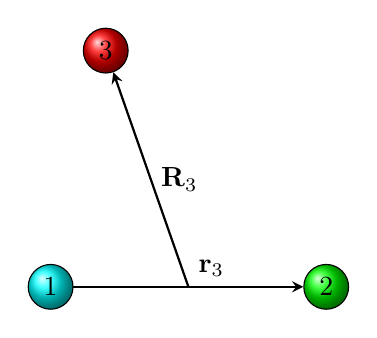
\begin{tikzpicture}[line cap = round, line join = round, >=triangle 45]
\tikzstyle{point1}=[ball color=cyan, circle, draw=black, inner sep=0.1cm]
\tikzstyle{point2}=[ball color=green, circle, draw=black, inner sep=0.1cm]
\tikzstyle{point3}=[ball color=red, circle, draw=black, inner sep=0.1cm]
\node[point1] (origin) at (0,0) {1};
\node[point2] (A) at (3.5,0)   {2};
\node[point3] (B) at (0.7, 3) {3};
\coordinate (M) at ($ (origin) !.5! (A) $);

\draw[thick,-stealth,color=black] (origin) -- (A) node[pos=0.6, above]{$\mathbf{r}_{3}$};
\draw[thick,-stealth,color=black] (M) -- (B) node[pos=0.5, right]{$\mathbf{R}_{3}$};
%\draw (1,0) arc (180:116:1);
\end{tikzpicture}
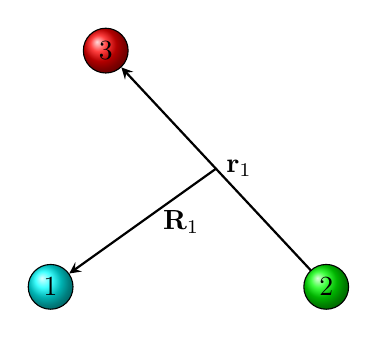
\begin{tikzpicture}[line cap = round, line join = round, >=triangle 45]
\tikzstyle{point1}=[ball color=cyan, circle, draw=black, inner sep=0.1cm]
\tikzstyle{point2}=[ball color=green, circle, draw=black, inner sep=0.1cm]
\tikzstyle{point3}=[ball color=red, circle, draw=black, inner sep=0.1cm]
\node[point1] (origin) at (0,0) {1};
\node[point2] (A) at (3.5,0)   {2};
\node[point3] (B) at (0.7, 3) {3};
\coordinate (M) at ($ (A) !.5! (B) $);

\draw[thick,-stealth,color=black] (A) -- (B) node[pos=0.5, right]{$\mathbf{r}_{1}$};
\draw[thick,-stealth,color=black] (M) -- (origin) node[pos=0.3, below]{$\,\,\,\,\mathbf{R}_{1}$};
\end{tikzpicture}
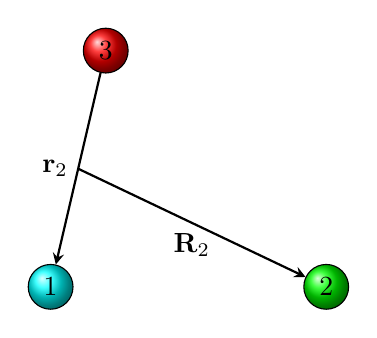
\begin{tikzpicture}[line cap = round, line join = round, >=triangle 45]
\tikzstyle{point1}=[ball color=cyan, circle, draw=black, inner sep=0.1cm]
\tikzstyle{point2}=[ball color=green, circle, draw=black, inner sep=0.1cm]
\tikzstyle{point3}=[ball color=red, circle, draw=black, inner sep=0.1cm]
\node[point1] (origin) at (0,0) {1};
\node[point2] (A) at (3.5,0)   {2};
\node[point3] (B) at (0.7, 3) {3};
\coordinate (M) at ($ (origin) !.5! (B) $);

\draw[thick,-stealth,color=black] (B) -- (origin) node[pos=0.5, left]{$\mathbf{r}_{2}$};
\draw[thick,-stealth,color=black] (M) -- (A) node[pos=0.5, below]{$\mathbf{R}_{2}$};
\end{tikzpicture}

\end{document}